\documentclass[12pt, twoside]{article}
\usepackage[letterpaper, margin=1in, headsep=0.5in]{geometry}
\usepackage[english]{babel}
\usepackage[utf8]{inputenc}
\usepackage{amsmath}
\usepackage{amsfonts}
\usepackage{amssymb}
\usepackage{tikz}
\usetikzlibrary{quotes, angles}
\usepackage{graphicx}
\usepackage{enumitem}
\usepackage{multicol}

\newif\ifmeta
\metatrue %print standards and topics tags

\title{Regents Geometry}
\author{Chris Huson}
\date{September 2020}

\usepackage{fancyhdr}
\pagestyle{fancy}
\fancyhf{}
\renewcommand{\headrulewidth}{0pt} % disable the underline of the header
\raggedbottom


\fancyhead[LE]{\thepage}
\fancyhead[RO]{\thepage \\ Name: \hspace{4cm} \,\\}
\fancyhead[LO]{BECA / Dr. Huson / Geometry 01-Intro\\* pset ID: 15}

\begin{document}

\subsubsection*{1-7HW-Calculations}
\begin{enumerate}
\item Given $\overline{ABC}$, $AB=84$, and $AC=116$.\\ [0.5cm]
  Find ${BC}$.\\[1.5cm]
      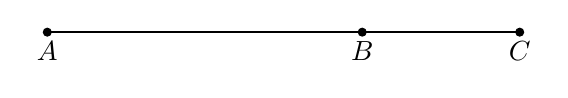
\begin{tikzpicture}
        \draw [-, thick] (1,0)--(7,0);
        \draw [fill] (1,0) circle [radius=0.05] node[below]{$A$};
        \draw [fill] (5,0) circle [radius=0.05] node[below]{$B$};
        \draw [fill] (7,0) circle [radius=0.05] node[below]{$C$};
      \end{tikzpicture} \vspace{2cm}

\item Given $\overline{DEF}$, $DE=7 \frac{1}{3}$, and $EF=3 \frac{1}{6}$. \\ [0.25cm]
  Find ${DF}$.\\[.5in]
      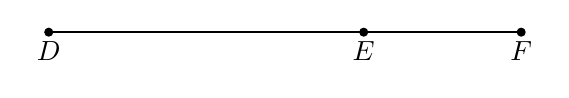
\begin{tikzpicture}
        \draw [-, thick] (1,0)--(7,0);
        \draw [fill] (1,0) circle [radius=0.05] node[below]{$D$};
        \draw [fill] (5,0) circle [radius=0.05] node[below]{$E$};
        \draw [fill] (7,0) circle [radius=0.05] node[below]{$F$};
      \end{tikzpicture} \vspace{2cm}

\item Given $\overleftrightarrow{PQ}$ as shown on the number line. \\[20pt] % Midpoint
    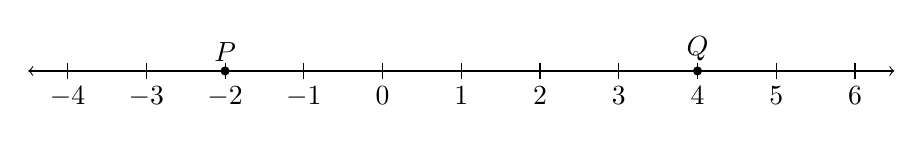
\begin{tikzpicture}
      \draw [<->] (-4.5,0)--(6.5,0);
      \foreach \x in {-4,...,6} %2 leading for diff!=1
        \draw[shift={(\x,0)},color=black] (0pt,-3pt) -- (0pt,3pt) node[below=5pt]  {$\x$};
        \draw [fill] (-2,0) circle [radius=0.05] node[above] {$P$};
        \draw [fill] (4,0) circle [radius=0.05] node[above] {$Q$};
    \end{tikzpicture} \\ \bigskip
    What is the exact distance on the number line between the points $P$ and $Q$? \vspace{1cm}  

\item Given $\overleftrightarrow{RS}$ as shown on the number line, with $R=0.7$ and $S=5.3$. \\[20pt]
    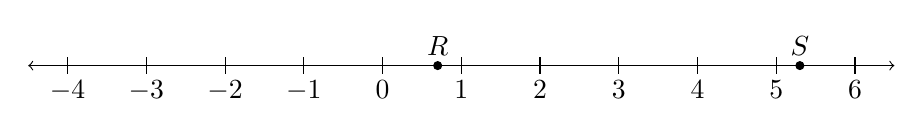
\begin{tikzpicture}
      \draw [<->] (-4.5,0)--(6.5,0);
      \foreach \x in {-4,...,6} %2 leading for diff!=1
        \draw[shift={(\x,0)},color=black] (0pt,-3pt) -- (0pt,3pt) node[below=5pt]  {$\x$};
        \draw [fill] (0.7,0) circle [radius=0.05] node[above] {$R$};
        \draw [fill] (5.3,0) circle [radius=0.05] node[above] {$S$};
    \end{tikzpicture} \\ \bigskip
    What is the distance on the number line between the points $R$ and $S$? \vspace{2cm}

\newpage
\item Given the rectangle $ABCD$ shown below, with $AB=11$ and $AD=5$. Find the area of the rectangle.
    \begin{flushleft}
    \begin{tikzpicture}
      \draw [-, thick] (0,0)--(7,0)--(7,4)--(0,4)--cycle;
      \draw [fill] (0,0) circle [radius=0.05] node[left]{$A$};
      \draw [fill] (7,0) circle [radius=0.05] node[right]{$B$};
      \draw [fill] (7,4) circle [radius=0.05] node[right]{$C$};
      \draw [fill] (0,4) circle [radius=0.05] node[left]{$D$};
      \node at (-0.5, 2){5};
      \node at (3.5, -0.5){11};
    \end{tikzpicture}
    \end{flushleft}

\item Given the rectangle $MATH$ shown below, with $MA=4.7$ and $MH=1.9$. Find the area of the rectangle.
    \begin{flushleft}
    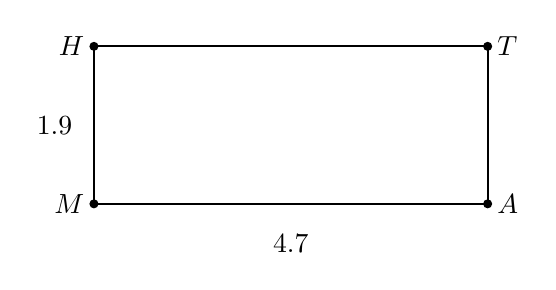
\begin{tikzpicture}
      \draw [-, thick] (0,0)--(5,0)--(5,2)--(0,2)--cycle;
      \draw [fill] (0,0) circle [radius=0.05] node[left]{$M$};
      \draw [fill] (5,0) circle [radius=0.05] node[right]{$A$};
      \draw [fill] (5,2) circle [radius=0.05] node[right]{$T$};
      \draw [fill] (0,2) circle [radius=0.05] node[left]{$H$};
      \node at (-0.5, 1){1.9};
      \node at (2.5, -0.5){4.7};
    \end{tikzpicture}
    \end{flushleft}
    \vspace{2cm}

\item In the following two problems, solve for the value of $x$.
  \begin{multicols}{2}
    \begin{enumerate}
      \item   $\frac{1}{2}(x+1)=-5$ \vspace{6cm}
      \item   $x-4.5=2.8-x$ \vspace{6cm}
    \end{enumerate}
  \end{multicols}
    \vspace{3cm}


\end{enumerate}
\end{document}